\documentclass{article}
\usepackage[utf8]{inputenc}
\usepackage[margin=1in]{geometry}
\usepackage{tikz}
\usepackage{pifont}
\usepackage{adjustbox}
\usetikzlibrary{shapes.geometric, arrows.meta, positioning, calc}

\begin{document}

\begin{figure}[htbp]
\centering
\begin{adjustbox}{max size={\textwidth}{\textheight}}
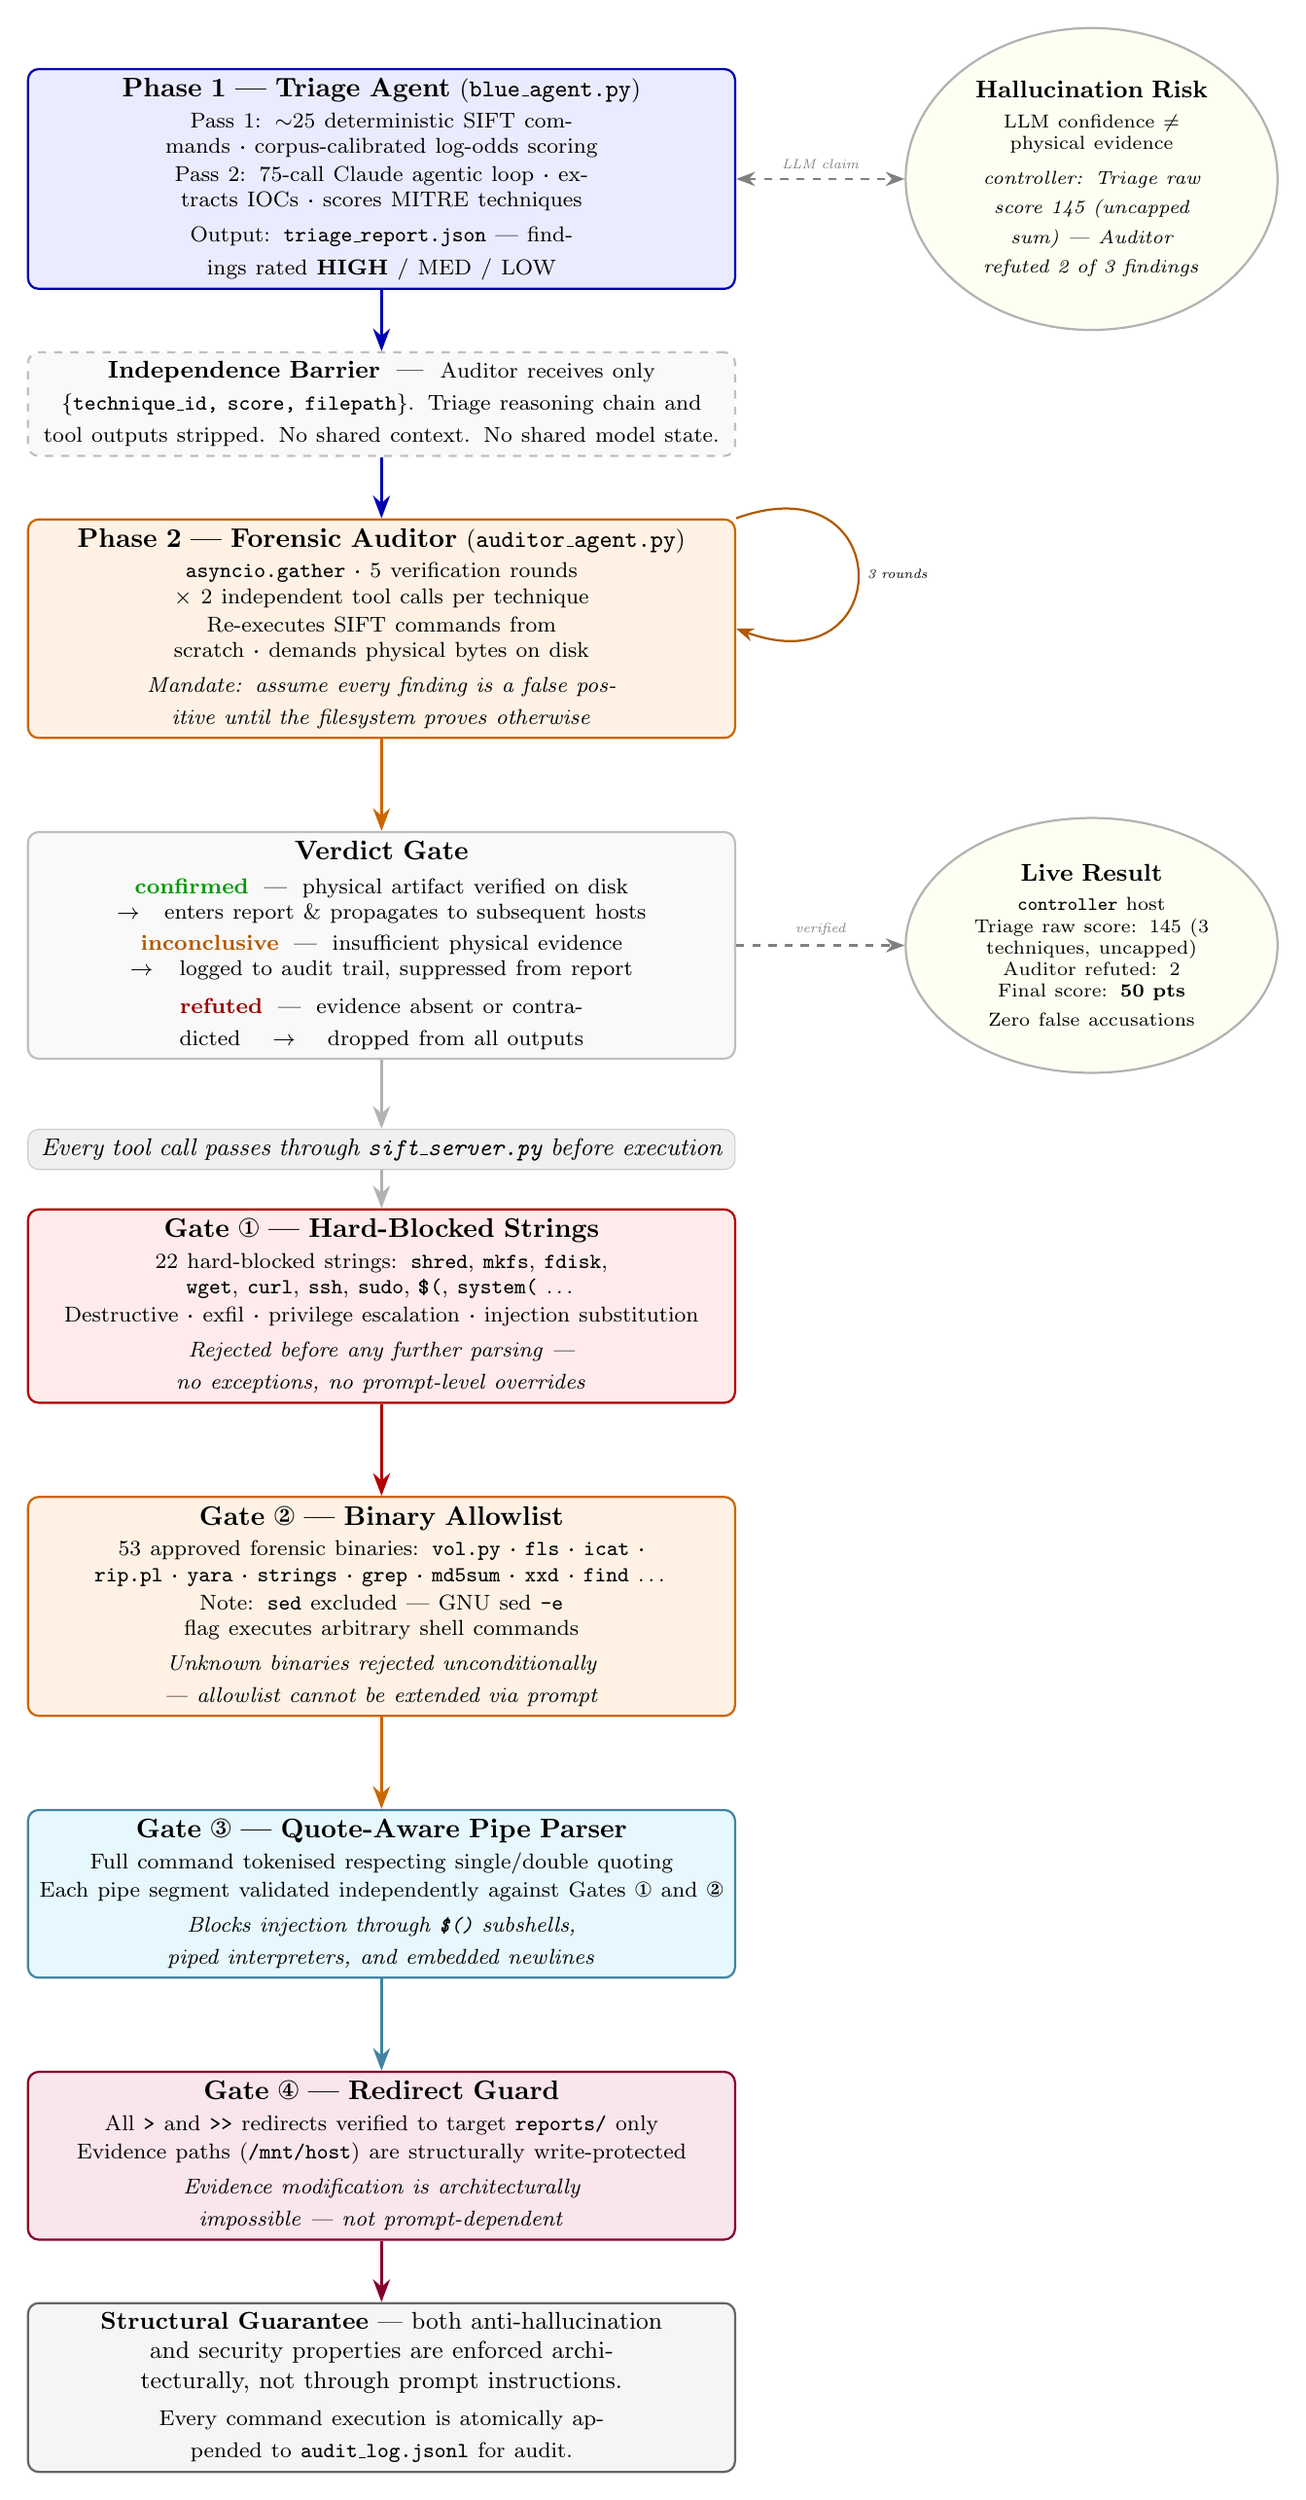
\begin{tikzpicture}[
    node distance=1.2cm,
    auto,
    >=Stealth,
    layer/.style={
        rectangle, draw=black, thick, fill=#1,
        text width=9cm, minimum height=1.4cm,
        align=center, rounded corners
    },
    barrier/.style={
        rectangle, draw=gray!50, dashed, thick, fill=gray!5,
        text width=9cm, minimum height=0.7cm,
        align=center, rounded corners
    },
    callout/.style={
        ellipse, draw=gray!60, fill=yellow!5, thick,
        text width=3.2cm, align=center, font=\small
    },
    arrow/.style={->, thick, line width=1.2pt}
]

    %% ═══════════════════════════════════════════════════════
    %% SECTION A — ANTI-HALLUCINATION TRUST CHAIN
    %% ═══════════════════════════════════════════════════════

    \node (triage) [layer=blue!8, draw=blue!70!black] {
        \textbf{Phase 1 — Triage Agent} \small(\texttt{blue\_agent.py}) \\[2pt]
        \footnotesize
        Pass 1: $\sim$25 deterministic SIFT commands · corpus-calibrated log-odds scoring \\[1pt]
        Pass 2: 75-call Claude agentic loop · extracts IOCs · scores MITRE techniques \\[1pt]
        Output: \texttt{triage\_report.json} — findings rated \textbf{HIGH} / MED / LOW
    };

    %% Hallucination risk callout (right of triage)
    \node (risk) [callout, right=2.2cm of triage] {
        \textbf{Hallucination Risk} \\[3pt]
        \scriptsize LLM confidence $\neq$ physical evidence \\[2pt]
        \textit{controller: Triage raw score 145 (uncapped sum) — Auditor refuted 2 of 3 findings}
    };

    \draw [<->, dashed, gray, line width=0.9pt]
        (triage.east) -- (risk.west)
        node[midway, above, font=\tiny\itshape] {LLM claim};

    %% ── Independence Barrier ──────────────────────────────
    \node (ind) [barrier, below=0.8cm of triage] {
        \textbf{\small Independence Barrier} \;—\;
        \footnotesize Auditor receives only \texttt{\{technique\_id, score, filepath\}}.
        Triage reasoning chain and tool outputs stripped.
        No shared context. No shared model state.
    };

    %% ── Forensic Auditor ─────────────────────────────────
    \node (auditor) [layer=orange!10, draw=orange!80!black, below=0.8cm of ind] {
        \textbf{Phase 2 — Forensic Auditor} \small(\texttt{auditor\_agent.py}) \\[2pt]
        \footnotesize
        \texttt{asyncio.gather} · 5 verification rounds $\times$ 2 independent tool calls per technique \\[1pt]
        Re-executes SIFT commands from scratch · demands physical bytes on disk \\[1pt]
        \textit{Mandate: assume every finding is a false positive until the filesystem proves otherwise}
    };

    %% Auditor re-verification self-loop
    \draw[->, thick, draw=orange!70!black]
        (auditor.north east)
        to [out=20, in=340, looseness=4]
        node[right, font=\tiny\itshape] {3 rounds}
        (auditor.east);

    %% ── Verdict Gate ─────────────────────────────────────
    \node (verdicts) [layer=gray!5, draw=gray!50, below=of auditor] {
        \textbf{Verdict Gate} \\[3pt]
        \footnotesize
        \textcolor{green!60!black}{\textbf{\textsc{confirmed}}} \;—\;
            physical artifact verified on disk
            $\;\rightarrow\;$ enters report \& propagates to subsequent hosts \\[2pt]
        \textcolor{orange!70!black}{\textbf{\textsc{inconclusive}}} \;—\;
            insufficient physical evidence
            $\;\rightarrow\;$ logged to audit trail, suppressed from report \\[2pt]
        \textcolor{red!60!black}{\textbf{\textsc{refuted}}} \;—\;
            evidence absent or contradicted
            $\;\rightarrow\;$ dropped from all outputs
    };

    %% Live result callout (right of verdicts)
    \node (result) [callout, right=2.2cm of verdicts] {
        \textbf{Live Result} \\[3pt]
        \scriptsize \texttt{controller} host \\
        Triage raw score: 145 (3 techniques, uncapped) \\
        Auditor refuted: 2 \\
        Final score: \textbf{50 pts} \\
        Zero false accusations
    };

    \draw [->, dashed, gray, line width=0.9pt]
        (verdicts.east) -- (result.west)
        node[midway, above, font=\tiny\itshape] {verified};

    %% ═══════════════════════════════════════════════════════
    %% SECTION B — MCP SECURITY BOUNDARY
    %% ═══════════════════════════════════════════════════════

    \node (sep) [
        rectangle, fill=gray!12, draw=gray!40,
        text width=9cm, minimum height=0.45cm,
        align=center, font=\small\itshape, rounded corners,
        below=0.9cm of verdicts
    ] {
        Every tool call passes through \texttt{sift\_server.py} before execution
    };

    %% ── Gate 1 ───────────────────────────────────────────
    \node (G1) [layer=red!8, draw=red!70!black, below=0.5cm of sep] {
        \textbf{Gate \ding{172} — Hard-Blocked Strings} \\[2pt]
        \footnotesize
        22 hard-blocked strings: \texttt{shred}, \texttt{mkfs}, \texttt{fdisk}, \texttt{wget},
        \texttt{curl}, \texttt{ssh}, \texttt{sudo}, \texttt{\$(}, \texttt{system(} \ldots \\[1pt]
        Destructive · exfil · privilege escalation · injection substitution \\[1pt]
        \textit{Rejected before any further parsing — no exceptions, no prompt-level overrides}
    };

    %% ── Gate 2 ───────────────────────────────────────────
    \node (G2) [layer=orange!10, draw=orange!80!black, below=of G1] {
        \textbf{Gate \ding{173} — Binary Allowlist} \\[2pt]
        \footnotesize
        53 approved forensic binaries:
        \texttt{vol.py} · \texttt{fls} · \texttt{icat} · \texttt{rip.pl} · \texttt{yara} ·
        \texttt{strings} · \texttt{grep} · \texttt{md5sum} · \texttt{xxd} · \texttt{find} \ldots \\[1pt]
        Note: \texttt{sed} excluded — GNU sed \texttt{-e} flag executes arbitrary shell commands \\[1pt]
        \textit{Unknown binaries rejected unconditionally — allowlist cannot be extended via prompt}
    };

    %% ── Gate 3 ───────────────────────────────────────────
    \node (G3) [layer=cyan!10, draw=cyan!60!black, below=of G2] {
        \textbf{Gate \ding{174} — Quote-Aware Pipe Parser} \\[2pt]
        \footnotesize
        Full command tokenised respecting single/double quoting \\[1pt]
        Each pipe segment validated independently against Gates \ding{172} and \ding{173} \\[1pt]
        \textit{Blocks injection through \texttt{\$()} subshells, piped interpreters, and embedded newlines}
    };

    %% ── Gate 4 ───────────────────────────────────────────
    \node (G4) [layer=purple!10, draw=purple!70!black, below=of G3] {
        \textbf{Gate \ding{175} — Redirect Guard} \\[2pt]
        \footnotesize
        All \texttt{>} and \texttt{>>} redirects verified to target \texttt{reports/} only \\[1pt]
        Evidence paths (\texttt{/mnt/host}) are structurally write-protected \\[1pt]
        \textit{Evidence modification is architecturally impossible — not prompt-dependent}
    };

    %% ── Structural Guarantee ─────────────────────────────
    \node (guarantee) [
        rectangle, draw=black!60, thick, fill=black!4,
        text width=9cm, minimum height=1.0cm,
        align=center, rounded corners,
        below=0.8cm of G4
    ] {
        \small\textbf{Structural Guarantee} —
        both anti-hallucination and security properties are enforced architecturally,
        not through prompt instructions. \\[2pt]
        \footnotesize
        Every command execution is atomically appended to \texttt{audit\_log.jsonl} for audit.
    };

    %% ── VERTICAL FLOW ARROWS ─────────────────────────────
    \draw [arrow, draw=blue!70!black]   (triage)   -- (ind);
    \draw [arrow, draw=blue!70!black]   (ind)      -- (auditor);
    \draw [arrow, draw=orange!80!black] (auditor)  -- (verdicts);
    \draw [arrow, draw=gray!60]         (verdicts) -- (sep);
    \draw [arrow, draw=gray!60]         (sep)      -- (G1);
    \draw [arrow, draw=red!70!black]    (G1)       -- (G2);
    \draw [arrow, draw=orange!80!black] (G2)       -- (G3);
    \draw [arrow, draw=cyan!60!black]   (G3)       -- (G4);
    \draw [arrow, draw=purple!70!black] (G4)       -- (guarantee);

\end{tikzpicture}
\end{adjustbox}
\caption{VERITAS Guardrails — Anti-Hallucination Trust Chain \& MCP Security Boundary}
\label{fig:adversa_guardrails}
\end{figure}

\end{document}
